\documentclass[conference]{./IEEEtran}

\usepackage{cite}
\usepackage[pdftex]{graphicx}
\usepackage{algorithmic}
\usepackage{hyperref}

% correct bad hyphenation here
\hyphenation{op-tical net-works semi-conduc-tor}


\begin{document}

\title{A proximity localization system for routing audio streams based on Bluetooth technology}
\author{Davide~Pesavento, Martina~Astegno \\
		Universit\`{a} degli Studi di Padova \\
		Corso di Laurea Magistrale in Informatica\\
		\{dpesaven,mastegno\}@studenti.math.unipd.it

}
%\author{\IEEEauthorblockN{Davide Pesavento}
%\IEEEauthorblockA{Universit\`{a} degli Studi di Padova\\
%Corso di Laurea Magistrale in Informatica\\
%Email: email@studenti.math.unipd.it}
%\and
%\IEEEauthorblockN{Martina Astegno}
%\IEEEauthorblockA{Universit\`{a} degli Studi di Padova\\
%Corso di Laurea Magistrale in Informatica\\
%Email: martina.astegno@studenti.unipd.it}}

% make the title area
\maketitle


\begin{abstract}
%\boldmath
We present in this paper an application that shows how the bluetooth technology can be used to locate a person who has a bluetooth device (e.g. smartphone) in a set of possible rooms.  The final aim is to playback an audio stream stored in a central server and move it from a speaker to an another, situated in every room, following person's movements.
\end{abstract}

\begin{IEEEkeywords}%normally used for peerreview paper
Bluetooth, Pulseaudio, conductor.
\end{IEEEkeywords}




% For peer review papers, you can put extra information on the cover
% page as needed:
% \ifCLASSOPTIONpeerreview
% \begin{center} \bfseries EDICS Category: 3-BBND \end{center}
% \fi
%
% For peerreview papers, this IEEEtran command inserts a page break and
% creates the second title. It will be ignored for other modes.
\IEEEpeerreviewmaketitle


%\hfill October 16, 2010

\section{Introduction}
\subsection{Bluetooth technology}
Bluetooth is an open specification for a radio system that provides the network infrastructure to enable short range wireless communication of data and voice. It comprises of a hardware component and a software component. The specification also describes usage models and user profiles for these models. 
Bluetooth supports two kinds of links: Asynchronous Connectionless (ACL) links for data transmission and Synchronous Connection oriented (SCO) links for audio/voice transmission. It uses Frequency Hoppping Spread Spectrum (FHSS) to avoid any interference. A bluetooth channel is divided into time slots each 625 micro second in length. The devices hop through these timeslots making 1600 hops per second. This trades bandwidth efficiency for reliability, integrity and security.
%In figure \ref{stack} we can see the architecture of bluetooth protocol.

In our project we adopt a specific Bluetooth stack implementation, \textbf{Bluez}, that provides support for the core Bluetooth layers and protocols. It is flexible, efficient and uses a modular implementation (Figure \ref{bluez}). \\
Currently BlueZ consists of many separate modules:
\begin{itemize}
\item Bluetooth kernel subsystem core
\item L2CAP and SCO audio kernel layers
\item RFCOMM, BNEP, CMTP and HIDP kernel implementations
\item HCI UART, USB, PCMCIA and virtual device drivers
\item General Bluetooth and SDP libraries and daemons
\item Configuration and testing utilities
\item Protocol decoding and analysis tools
\end{itemize}
%bisogna trovare un immagine con lo stack BlueZ
%\begin{figure}[h]
%\centering
%\includegraphics[scale = 0.7]{bluezDef.png}
%\caption{Bluez Overview diagram}
%\label{bluez}
%\end{figure}


\subsection{PulseAudio Server}
PulseAudio is a sound server for POSIX and Win32 systems. A sound server is basically a proxy for sound applications. It allows to do advanced operations on sound data as it passes between an application and the hardware. Things like transferring the audio to a different machine, changing the sample format or channel count and mixing several sounds into one are easily achieved using a sound server. In this context the main functionalities used are the audio stream control, to transfer the sound between different speakers according to the person movement and the simoultaneously playback from two or more speakers.  

\section{General architecture}

\subsection{Project requirements}
Before starting with the project design stage, we pointed out some basic requirements for the project. Here, we propose a list and a description for the main ones.
\begin{itemize}
\item{\textbf{Smartphone:}} the device necessary to locate in which room the person is. We assume that there is only one smartphone to identify.  
\item{\textbf{Central server:}} it stores the main application and it controls all the communications from/to the BT adapter.
\end{itemize}
In every room there must be available:
\begin{itemize}
\item{a \textbf{bluetooth host adapter:}} it detects the bluetooth signal power, and trasmits throught a simple application the RSSI value to the central server; 
\item{a \textbf{speaker:}} it lets out sound when the associate bluetooth adapter is selected for playback.
\end{itemize}

%immagine con la architettura ad alto livello che mostra come interagiscono le componenti
\begin{figure}[h]
\centering
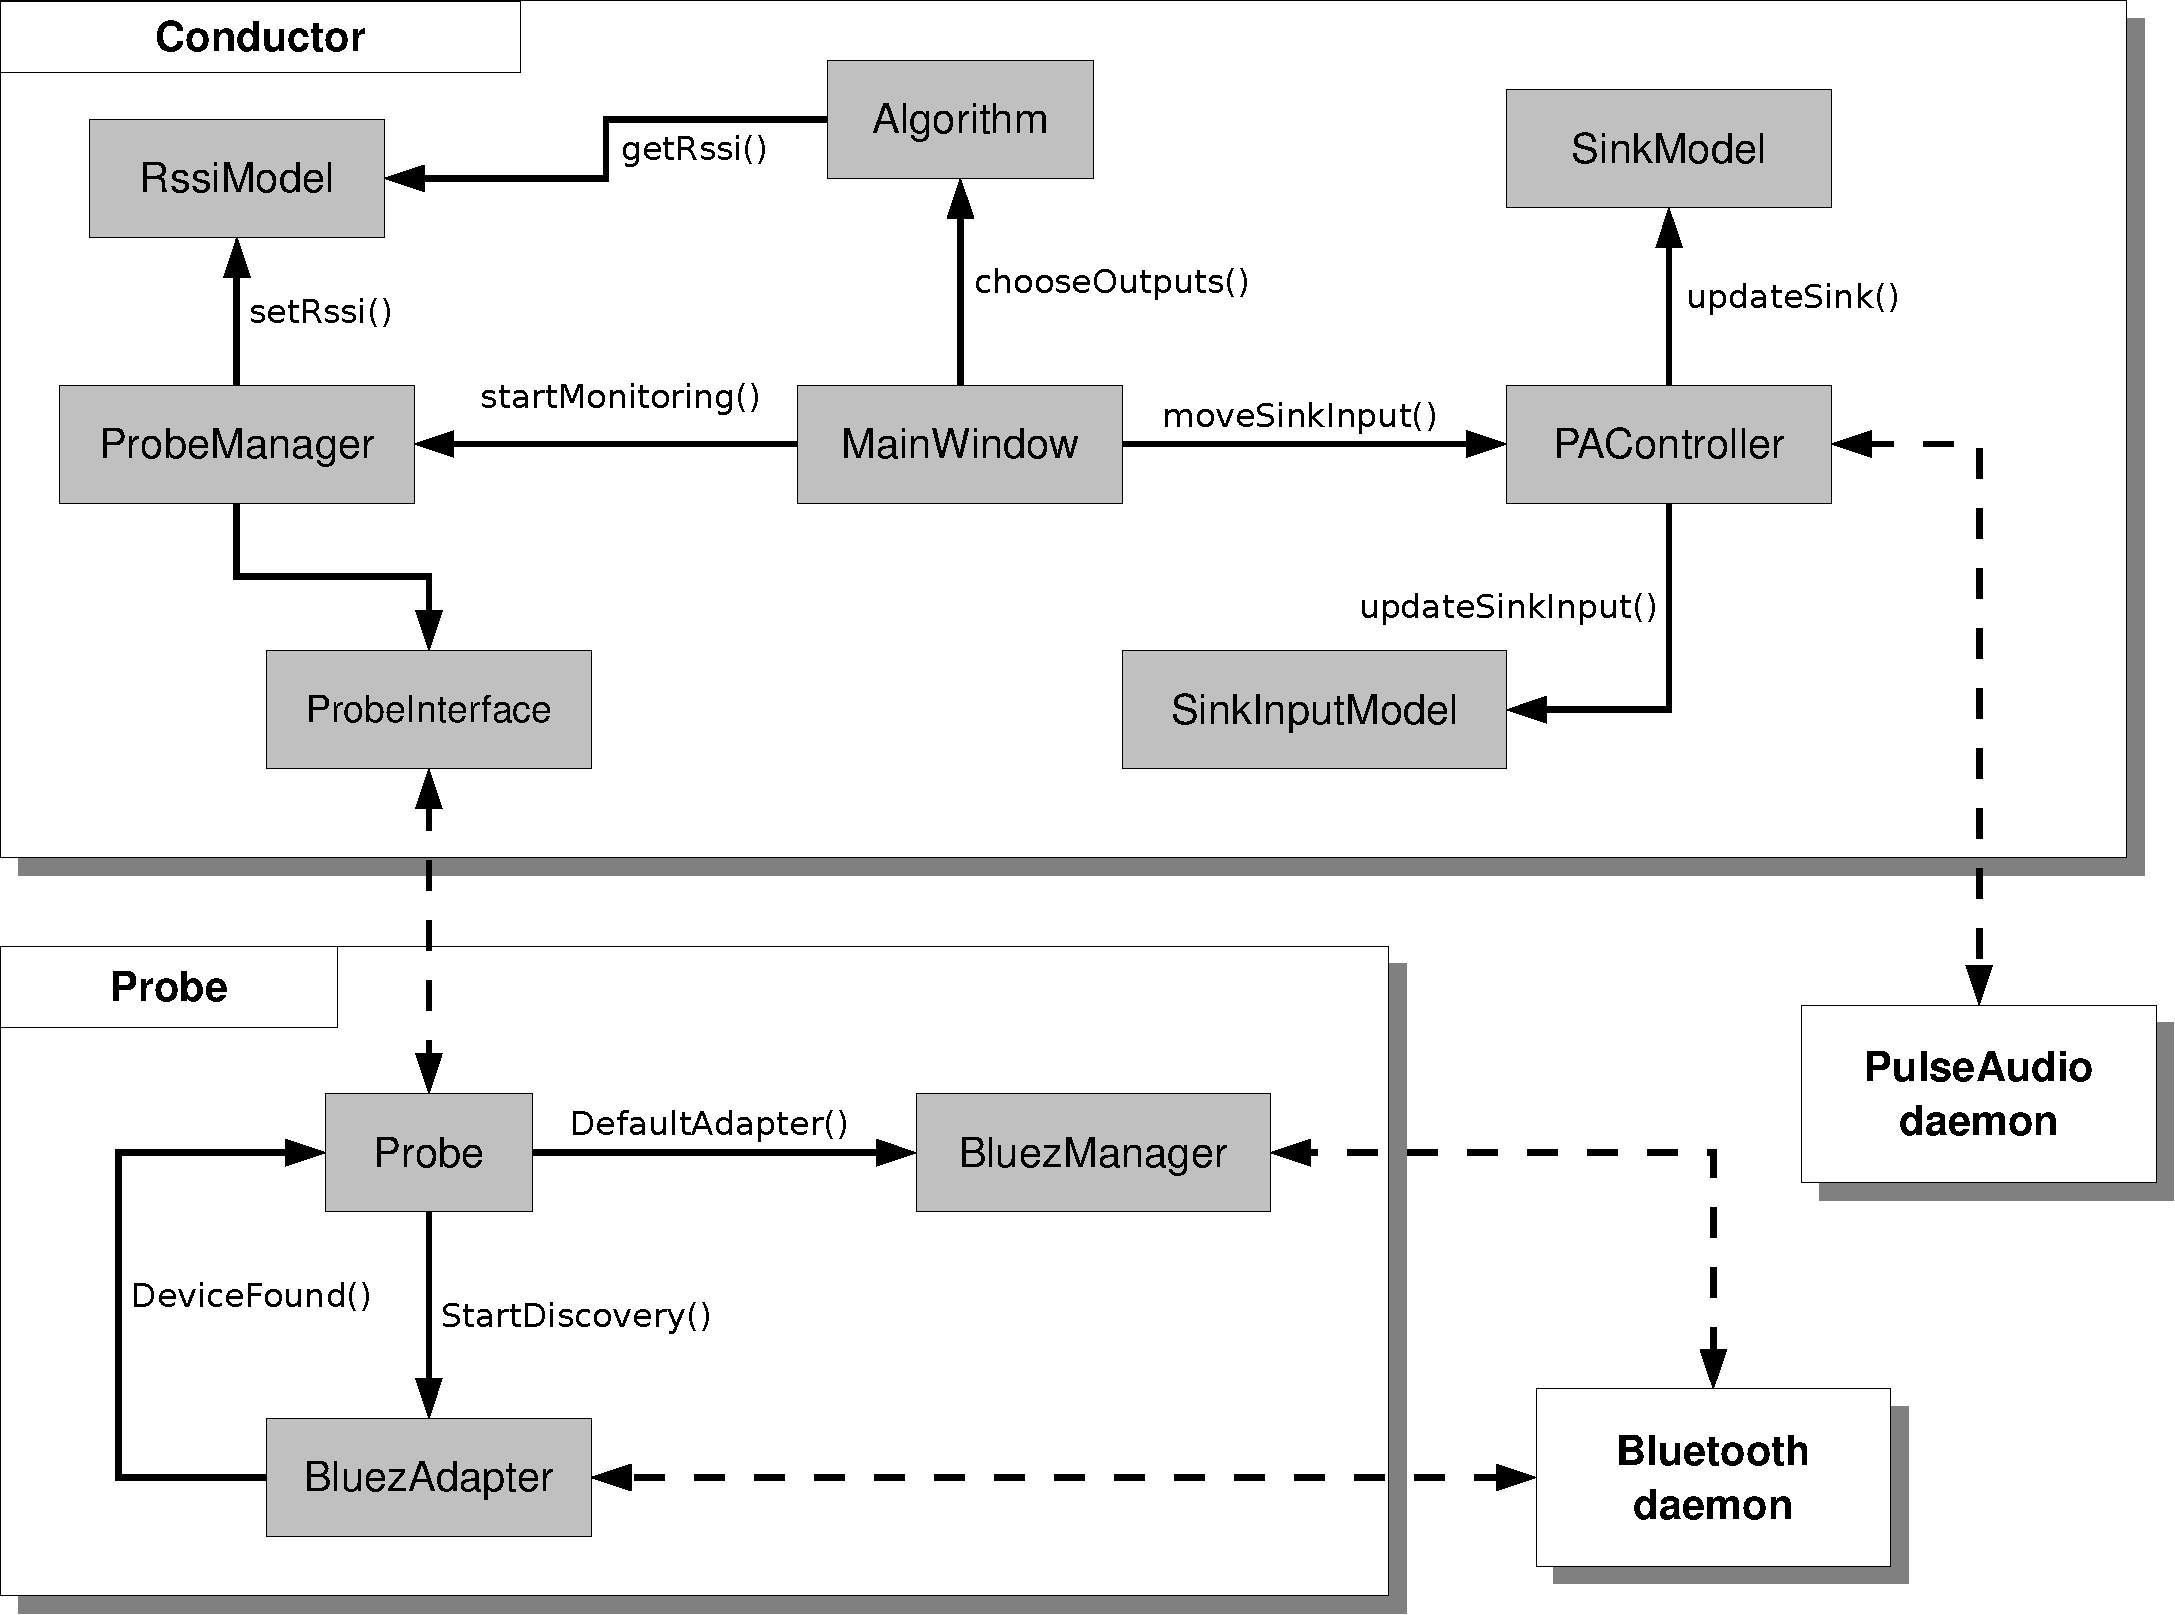
\includegraphics[scale = 0.3]{architettura.pdf}
\caption{Interaction between components}
\label{arch}
\end{figure}


\subsection{Bluetooth module}
The main component of the project is the Bluetooth module, that manages the RSSI values and communications between bluetooth hosts and device. It is based on a simple and very efficient application, named Probe and associated to every bluetooth host adapter, that is able to interface with \textbf{bluez} throught \textbf{d-bus}. In details, every bluetooth adapter is modeled by the class \texttt{ProbeInterface} that allows to manage a start or stop discovery request done by the device and to update the RSSI values when a change occurs. All the \texttt{ProbeInterface} objects are controlled by the class \texttt{ProbeManager} that monitors the device localization and stores the information about every \texttt{ProbeInterface} (e.g. the name room associated with the adapter).     

\subsection{Pulseaudio module}
In Pulseaudio we distinguish two particolar types of structures managed in our application.
\begin{itemize}
\item \texttt{pa\_sink}: 
\item \texttt{pa\_sink\_input}:
\end{itemize}
To control and monitor the PulseAudio operations we implemented the class \texttt{pacontroller}. There are two main methods:
\begin{itemize}
\item \texttt{PAController::createTunnel(const QByteArray )}
\item \texttt{PAController::combineSinks(const QList<uint32\_t>, const QString, int, const QString}
\end{itemize} 
The first method allows to create a sink that acts as tunnel connection with the server specified in the parameter in which it's running a PulseAudio daemon. When it's available the complete list of sinks, we can redirect the \texttt{pa\_sink\_input} coming from a specific application (e.g. MPlayer) to one or more sinks associated with a speaker in every room. In PulseAudio this operation is done loading a particular module called \texttt{<module-tunnel-sink>}. 
By default the audio is reproduced by only one \texttt{pa\_sink}. With the second method it is possible to playback sound throught more speakers simultaneously, loading the PulseAudio \texttt{<module-combine>} that combines more objects \texttt{pa\_sink} creating a new sink with a specified identifier.  


\subsection{Algorithm}
The algorithm implemented determines which speaker has to playback sound according to person's location; we can suppose infact that the signal power detected by the bluetooth adapter is higher than the other RSSI values in the room where person is situated. The following pseudo-code shows how the algorithm works. The output returned represents the index of speakers/rooms where the sound has to be reproduced.

Input variables:
\begin{itemize}
\item \textbf{retryCount}: the time spent from inizialization to the request of available RSSIs.
\item \textbf{maxRetries}: the threshold that when exceeded the playback is forced to start, even if there aren't all data available.
%\item \textbf{sortedRssi}: the map with every devices, sorted by the RSSI value associated with each ones. 
\item \textbf{curRooms}: it's a set that contains the addresses of rooms in which the playback occurs in the current moment.
%\item \textbf{No\_null\_RSSI}: number of available RSSI values.
\item \textbf{adjacencyMap}: the map stores the list of adjoining rooms for every specific room.   
\item \textbf{rssiMap}: it stores for every bluetooth adapter the RSSI value detected.
%\item \textbf{minNumberRssi}: min number of RSSI required to proceed with the sound playback. 
\item \textbf{maxSimultaneousSpeakers}: max number of speakers that can be activated simultanously.
\end{itemize}
\textbf{\underline{ChooseOutputs algorithm:}}
\vspace{0.3cm}
\begin{algorithmic}[1]

\STATE $outputs \gets null$ \COMMENT{Create the variable to return the list of speakers to activate for playback}
\STATE $retryCount \gets 0$
\STATE $sort$ $(rssiMap)$ \COMMENT{Sort the RSSI values} 

\STATE $results \gets null$
\FOR{$i = 1$ to $ maxSimultaneouslySpeakers$}
\STATE $results \gets results$ $\cup$ $rssiMap$ $(i)$ \COMMENT{Choose the rooms with highest RSSI with UB and insert them into $results$}
\ENDFOR

\IF{($results$ is empty) \textbf{and} ($retryCount < maxRetries$)}
\STATE $ retryCount \gets retryCount + 1 $ \COMMENT{Wait a bit more if we don't have enough data}
\STATE GOTO 3)
\ENDIF

\FOR{$i = 1$ to $ numElements$ $(results)$} 
	\IF{$ results(i) \in adjacencyMap$ $(curRooms)$} 
		\STATE $outputs \gets outputs$ $\cup$ $results(i)$ \COMMENT{Add element after intersection with rooms contiguous to the current ones}
	\ENDIF
\ENDFOR
\RETURN outputs
\end{algorithmic}
%In the algorithm just exposed the method \texttt{add(Object[] param1, Object param2)} symple adds \texttt{param2} to the list contains in \texttt{param1}.

%\subsection{Tester}
%bisogna mettere che i dati sono precompilati, perchè non avevamo l'HW adatto che fornisse i lvalore di RSSI in seguito a d una inquiry.

\section{Runtime behavior}

\subsection{Configuration}
Before starting the application it is necessary to setup some parameter in the configuration file. The information to provide are:
\begin{itemize}
\item \texttt{maxRetries}: it represents a threshold. When crossed the playback is forced to start. 
\item \texttt{maxSimultaneousSpeakers}: the max number of speakers activated at the same time.
\item \texttt{probesAddresses}: the IP addresses of Probes associated with each room.
\item \texttt{roomsNames}: the names associated with each room.
\item \texttt{roomsTopology}: it describes the relative localization of each room. %respect to each other. 
\end{itemize}

\subsection{Monitoring}


\section{Experiments Evaluation}

\section{Future work and conclusion}
Here we will explain some possible project extensions. 
\subsection{Improve testing phase}
Currently our application has been tested using an additional component that simulates the person movements. In detail it is a particular interface (a button) associated with each Probe application. By clicking it we can increase the RSSI value associated with the respective adapter and consequently decrease the RSSI values associated with the other adapters. However being only a simulation, the behavior doesn't match totally with the real one.  
\subsection{Multiple devices}
Although an assumption of the present project is the identification of a single smartphone. It would be important to allow the application to support and manage multiple devices. This entails the necessity to consider how different devices could interact and interfere between them.       
\subsection{``Mixer'': Application on device}
In our project the main application runs in the central server. The device (smartphone) is only used to localize the person. It would be interesting to develop an application for the smartphone to give the user a certain control on the audio stream. For instance with this new feature the person should be able to regulate the volume and to stop the playback. A further improvement could be an interface to navigate through the playlist, i.e. choose a specific song or skip to the previous/next track.  


% conference papers do not normally have an appendix


% use section* for acknowledgement
%\section*{Acknowledgment}


%The authors would like to thank...





% trigger a \newpage just before the given reference
% number - used to balance the columns on the last page
% adjust value as needed - may need to be readjusted if
% the document is modified later
%\IEEEtriggeratref{8}
% The "triggered" command can be changed if desired:
%\IEEEtriggercmd{\enlargethispage{-5in}}

% references section

% can use a bibliography generated by BibTeX as a .bbl file
% BibTeX documentation can be easily obtained at:
% http://www.ctan.org/tex-archive/biblio/bibtex/contrib/doc/
% The IEEEtran BibTeX style support page is at:
% http://www.michaelshell.org/tex/ieeetran/bibtex/
%\bibliographystyle{IEEEtran}
% argument is your BibTeX string definitions and bibliography database(s)
%\bibliography{IEEEabrv,../bib/paper}
%
% <OR> manually copy in the resultant .bbl file
% set second argument of \begin to the number of references
% (used to reserve space for the reference number labels box)
\begin{thebibliography}{1}
\bibitem{Pulseaudio} 
		PulseAudio Sound Server, 
		\url{http://www.pulseaudio.org/}
\bibitem{Bluez} 
		BlueZ: Official Linux Bluetooth protocol stack, 
		\url{http://www.bluez.org/}


%\bibitem{IEEEhowto:kopka}
%H.~Kopka and P.~W. Daly, \emph{A Guide to \LaTeX}, 3rd~ed.\hskip 1em plus
 % 0.5em minus 0.4em\relax Harlow, England: Addison-Wesley, 1999.

\end{thebibliography}




% that's all folks
\end{document}


